%% NM x Lang x Op:
%% Reduct x UntypedLambda x eval
\subsection{Reduct}
\label{sec:Reduct}

% \begin{meta}
% \begin{itemize}
%     \item Describe it (try to describe it in a way that is faithful to the implementation) \done
%     \item Explain motivations of the design (they wanted to make it like a game and "repetition" was added to make it interesting) \done
%     \item Show examples \done
%     \item Show possible implementation attempt (the one that is wrong). There is no correspondence between an application node and 
%     \item Describe how it relates to the language (an informal description of $\alpha$)
%     \item Try to build the commutation diagram and explain how that leads to detecting inconsistency
%     \item Explain the problem: Inconsistency already comes up in the creation of $\alpha$ (the mapping from lang to NM)
%     \item show example of program that cannot be built
%     \item Propose solution: how can the datastructure of the abstract NM could be adapted. What are the implications?
%     \item build the diagram for implementation of the adapted NM \done
%     \item explain diagram
% \end{itemize}
% \end{meta}

\Nms{} can serve as a basis for educational games.
One such example is Reduct,
an online game to teach ``core programming concepts
which include functions, Booleans, equality, conditionals, and mapping functions over sets''~\cite{arawjoTeachingProgrammingGamified2017}.
Reduct aims to represent a subset of JavaScript ES2015.
The gameplay of Reduct tightly interleaves program construction and program evaluation.
Each level of the game has a goal: to reduce terms to an expected value.
Within a level, at any point in time, the canvas contains a given number of independent
game pieces that correspond to terms in JavaScript.
The player clicks and drops these game pieces on each other both to compose them and to "reduce" them
(reduce the terms they correspond to).


\begin{table}
\begin{tabular}{|l||l|c|}
\hline
      & Programming Language & Notional Machine \\
      & \emph{JavaScript terms}     & \emph{Reduct pieces} \\
\hline
\hline
Literal value & \texttt{"star"}, \texttt{"triangle"}, and \texttt{"square"} & \begin{tabular}{c}
\includegraphics[scale=0.4]{images/reduct/Reduct-Star.png}, 
\includegraphics[scale=0.4]{images/reduct/Reduct-Triangle.png}, and 
\includegraphics[scale=0.4]{images/reduct/Reduct-Square.png}\end{tabular} \\
\hline
Boolean     & \verb|true| or \verb|false| & \begin{tabular}{c}
\includegraphics[scale=0.4]{images/reduct/Reduct-Key.png} or 
\includegraphics[scale=0.4]{images/reduct/Reduct-KeyBroken.png}\end{tabular} \\
\hline
Conditional & \verb|x ? y : null|         & \begin{tabular}{c}
\includegraphics[scale=0.4]{images/reduct/Reduct-Lock.png}\end{tabular} \\
\hline
Comparison  & \verb|x == y|               & \begin{tabular}{c}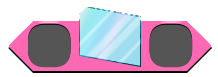
\includegraphics[scale=0.4]{images/reduct/Reduct-Mirror.png}\end{tabular} \\
\hline
Variable    & \verb|x|                    & \begin{tabular}{c}
\includegraphics[scale=0.4]{images/reduct/Reduct-var.png}\end{tabular} \\
\hline
Abstraction & \verb|x => t|               & \begin{tabular}{c}
\includegraphics[scale=0.4]{images/reduct/Reduct-abs.png}\end{tabular} \\
\hline
\multirow{5}{*}{Variations on Abstraction}  & \verb|x => x| & \begin{tabular}{c}
\includegraphics[scale=0.4]{images/reduct/Reduct-abs-1var.png}\end{tabular} \\
\cline{2-3}
                          & \verb|x => [t1, t2]| & \begin{tabular}{c}
\includegraphics[scale=0.4]{images/reduct/Reduct-abs-2plate.png}\end{tabular} \\
\cline{2-3}
                          & \verb|x => [x, x]| & \begin{tabular}{c}
\includegraphics[scale=0.4]{images/reduct/Reduct-abs-2var.png}\end{tabular} \\
\cline{2-3}
                          & \verb|x => [x, x, x]| & \begin{tabular}{c}
\includegraphics[scale=0.4]{images/reduct/Reduct-abs-3var.png}\end{tabular} \\
\cline{2-3}
                          & \verb|x => x == x| & \begin{tabular}{c}
\includegraphics[scale=0.4]{images/reduct/Reduct-abs-var-eq-var.png}\end{tabular} \\
\hline
\end{tabular}
\caption{Metaphors used in \nmName{Reduct}}
\label{tab:reduct}
\end{table}

Like other \nms{}, \nmName{Reduct} employs metaphors
to allow learners to reuse their understanding of the real world
when learning the semantics of the programming language.
Table~\ref{tab:reduct} shows some of \nmName{Reduct}'s metaphors\footnote{Reduct introduces the idea of ``concreteness fading'':
while progressing through the levels of the game, the pieces a player gets to use become gradually more abstract.
At the start, at the most concrete end of the spectrum, Reduct uses the metaphors described above.
In the end, at the most abstract end of the spectrum, it uses blocks that essentially contain JavaScript code.}.
%
Star, square, and triangle \emph{shapes} represent the literal String values \texttt{"star"}, \texttt{"square"}, and \texttt{"rectangle"}.
A \emph{key} represents the Boolean value \texttt{true}, and a \emph{broken key} represents \texttt{false}.
A \emph{lock} that protects a term represents a conditional operator.
The lock's keyhole takes on a condition (a term that produces a key).
The term protected by the lock corresponds to the term to evaluate if the condition holds;
the value produced if the condition does not hold, \texttt{null}, is not visually represented.
A \emph{reflecting glass}, with space for a term on either side, represents the equality operator.
A \emph{metal plate} represents a lambda abstraction:
the circular hole on its left represents the variable binding,
and the other hole on its right holds the lambda's body.
A \emph{pipe} that sticks out of the canvas represent variable use.
A value dropped in the metal plate's circular hole materializes in each of the pipes connected to the plate.

While a metal plate with a hole and a pipe are two separate constructs in some levels of the Reduct game,
most often they are inseparably connected.
We will refer to this combination of one or more pipes connected to a plate with a hole as a \emph{HolePipe}.

\subsubsection{Illustrative Example}
Figure~\ref{fig:reductA} shows the step-by-step solution of level 17 of the Reduct game\footnote{\url{https://www.therottingcartridge.com/games/programming/?level=17}}.
% terms described in the Reduct lang, not in lambda calculus
In Step 1, the canvas contains three independent pieces:
a HolePipe, a star, and a reflecting glass.
The goal of this level, shown in the top left corner, is to produce a key.
%
To make progress, the player should grab the star and drop it into the HolePipe's hole.
This results in the HolePipe and the star disappearing, and two stars (one for each pipe) appearing.
That step is supposed to correspond to the application of a lambda to a term.
% stop sign
This correspondence is not accurate, as we will show.
% or is it the other way around?
In steps 2 and 3, the player should plug the stars into the holes around the reflecting glass,
which triggers the evaluation of the comparison and produces a key.
That step corresponds to reducing the term \verb|"star" == "star"| to obtain \verb|true|.
%
%
% This step illustrates a key problem with \nmName{Reduct}:
% the absence of a separate construct for function application,
% and the confusion of function applications, as they are hard-wired into the bodies of lambdas,
% with a bunch of independent terms.
% Step 1 illustrates this problem:
% The two pipes in the lambda's body could be interpreted as a function application \verb|x x|
% (or \verb|x(x)| in JavaScript).
% Applying this lambda to the star should thus produce one JavaScript term, 
% \verb|"star"("star")|.
% However, in \nmName{Reduct}, applying this lambda produces not one but \textit{two} independent terms,
% \verb|"star"| and \verb|"star"|.
%
%

% \begin{figure}
%     \centering
%     \begin{tabular}{lllll}
%         Step 1                             & Step 2        & Step 3             & Step 4                  & Step 5 \\
%         \verb|x => x x| \textit{(problem)} & \verb|"star"| &                    &                         & \\
%         \verb|"star"|                      & \verb|"star"| & \verb|"star"|      &                         & \\
%         \verb|y == z|                      & \verb|y == z| & \verb|"star" == z| & \verb|"star" == "star"| & \verb|true| \\
%         \includegraphics[scale=0.08]{images/lambda_xdot_x_x_-_y_eq_z_-_a_-_1.png} &
%         \includegraphics[scale=0.08]{images/lambda_xdot_x_x_-_y_eq_z_-_a_-_2.png} &
%         \includegraphics[scale=0.08]{images/lambda_xdot_x_x_-_y_eq_z_-_a_-_3.png} &
%         \includegraphics[scale=0.08]{images/lambda_xdot_x_x_-_y_eq_z_-_a_-_4.png} &
%         \includegraphics[scale=0.08]{images/lambda_xdot_x_x_-_y_eq_z_-_a_-_5.png} \\
%     \end{tabular}
%     \caption{Evaluation in programming language (top) and \nmName{Reduct} \nm{} (bottom).}
%     \label{fig:reductA-old}
% \end{figure}
% \todo make this image more visible by increasing the game board in each step.
\begin{figure}
    \centering
    \begin{tabular}{|l|p{4.5cm}|l|}
    \hline
    Step & Programming Language & \NM{} \\\hline
    \hline
    1 & \verb|x => x x|, \verb| "star"|, \verb| y == z| & \includegraphics[scale=0.15]{images/reduct/lambda_xdot_x_x_-_y_eq_z_-_a_-_1.png} \\\hline
    \multicolumn{3}{c}{drag and drop star into plate's round hole} \\\hline
    2 & \verb|"star"|, \verb| "star"|, \verb| y == z|   & \includegraphics[scale=0.15]{images/reduct/lambda_xdot_x_x_-_y_eq_z_-_a_-_2.png} \\\hline
    \multicolumn{3}{c}{drag and drop star into hole left of reflecting glass} \\\hline
    3 & \verb|"star"|, \verb| "star" == z|              & \includegraphics[scale=0.15]{images/reduct/lambda_xdot_x_x_-_y_eq_z_-_a_-_3.png} \\\hline
    \multicolumn{3}{c}{drag and drop star into hole right of reflecting glass} \\\hline
    4 & \verb|"star" == "star"|                         & \includegraphics[scale=0.15]{images/reduct/lambda_xdot_x_x_-_y_eq_z_-_a_-_4.png} \\\hline
    \multicolumn{3}{c}{click on reflecting glass} \\\hline
    5 & \verb|true|                                     & \includegraphics[scale=0.15]{images/reduct/lambda_xdot_x_x_-_y_eq_z_-_a_-_5.png} \\\hline
    \end{tabular}
    \caption{Evaluation in programming language (left) and \nmName{Reduct} \nm{} (right).}
    \label{fig:reductA}
\end{figure}

%\Igor{\todo adapt text consistently with the new table}

\subsubsection{Commutative Diagram}
% problem
The first step is to define \ensuremath{\Conid{A}_{\Conid{NM}}}, \ensuremath{\Conid{A}_{\Conid{PL}}},
and a mapping $\alpha$ from \ensuremath{\Conid{A}_{\Conid{PL}}} to \ensuremath{\Conid{A}_{\Conid{NM}}}.
%
%
\ensuremath{\Conid{A}_{\Conid{PL}}} should be a type representing the terms of a subset of JavaScript as described in the paper,
but for convenience, we will focus on a subset of terms that is effectively equivalent to the untyped lambda-calculus.
Because of that, we can define \ensuremath{\Conid{A}_{\Conid{PL}}} to be \ensuremath{\Conid{Term}_{\Conid{U}\lambda}}.
%
Let's define \ensuremath{\Conid{A}_{\Conid{NM}}} to be \ensuremath{\Conid{ReductTerm}}, a type representing the constructs in \nmName{Reduct}.
We will consider just the constructs that correspond (as closely as possible) to the terms represented with \ensuremath{\Conid{Term}_{\Conid{U}\lambda}}.
%
%
% As we model \ensuremath{\Conid{A}_{\Conid{NM}}} let's try to create the mapping $\alpha$.
%
Our first construct to consider is the 
HolePipe, which corresponds to a lambda abstraction.
% , where
%JJ: I think this is a duplication. 
%The hole corresponds to a variable definition in a lambda abstraction
%and the pipes corresponds to a variable use.
% A value dropped in the hole materializes in each of the connected pipes.

The first thing to notice is that a HolePipe can contain multiple pipes next to each other,
as shown in Figure~\ref{fig:reductA}.
The effect of these
pipes is simply to create more occurrences of the term that is dropped in the hole.
This construct has no direct equivalent in the lambda-calculus, because
placing a term in front of another means application in lambda-calculus
and not "multiple returns".
%
Perhaps pipes next to each other could correspond to some kind of list term on the language level
so we would have to augment the language to add a term for that.
%
But we don't need to worry about this mismatch.
%
In itself, this mismatch is not a problem.
It is still possible to have a commutative diagram if there are constructs in \ensuremath{\Conid{A}_{\Conid{NM}}} that cannot be directly mapped to \ensuremath{\Conid{A}_{\Conid{PL}}}.
%
What is really missing in Reduct is a construct corresponding to function application.
The intention of the authors was to represent function application by dropping a term into the hole of a HolePipe construct.
%
When a term is dropped in the hole of a HolePiple, the HolePiple and the dropped term are replaced by as many copies of the dropped term as there are pipes in the HolePipe.
% important!
That would correspond to application, but more precisely it corresponds to the operational behavior of an application, not to the construction of an application term.
Constructing an application term is not the same as applying it immediately.
%

% example of term that can't be constructed
Without an application term, it is impossible to write several kinds of programs.
The Y-combinator, for example, which is used to construct recursive programs,
contains application terms, and
an essential part of its behavior is that, during execution,
the terms that are part of these application terms will be substituted to different terms as the recursion unfolds.
%
In general,
there are several kinds of programs that contain application terms $t_1\ t_2$ where $t_1$ and $t_2$
cannot be statically known but depend on the runtime behavior of the program.

% how did they "get away with this"?
Notably, this mismatch between the \nm{} and the programming language is not evident 
because the only ``programs'' one can write using Reduct
are the ones made out of the building blocks provided in each level of the game.
Effectively, the gameplay is a form of ``puzzle solving'' that corresponds to a mix of \emph{constructing} and \emph{reducing} terms.
In a programming language, however, one does not modify the program during its execution.

% solution
To solve this mismatch,
we need to not only add a construct in Reduct that corresponds to application,
but we need also to adapt the way the player interacts with the game to ``solve the puzzle''.
% 
Adding a construct in Reduct is simple.
More challenging is adapting the gameplay.
Part of the challenge is that
once programs are constructed, the only way a player should be able to interact with it to produce a given final result is by providing inputs.
%
At the same time, we don't want to lose the stepwise reduction of terms triggered by the player, which can be very instructive.
%
For this, there should be a way to distinguish between the moment when a program is built and the moment the program is run.
This distinction could be directly controlled by the player, who could explicitly say when the program is ready.
If a program does not depend on inputs, it can be run directly by clicking on the term to trigger reduction steps (similar to the current behavior).
Programs that depend on inputs could, for simplicity, be expressed as terms where the root is a lambda abstraction.
To run these programs,
the player would drop a term into the outermost lambda and subsequently click to trigger the next reduction steps.
An important difference from the current gameplay is that once a term is being executed it cannot be changed and a ``reset'' button would be needed to show the initial state of the program in case the desired final term is not reached.

In essence,
it is not possible to construct a mapping $\alpha$ from
\ensuremath{\Conid{Term}_{\Conid{U}\lambda}}
to an abstract representation of \nmName{Reduct}
because a lambda application node
does not have an adequate correspondence in \nmName{Reduct}.


% \[
% \begin{tikzcd}
% \operatorname{ReductTerm} \arrow[rrr, "\mathit{map} \alpha\; \circ\; \mathit{map} \operatorname{step}\; \circ\; \alpha^{\circ}", dashed] \arrow[ddd, "\alpha^{\circ}", shift left, dotted] & & & \operatorname{Maybe} \operatorname{ReductTerm} \\
%                                                           \\
%                                                           \\
% \operatorname{Term_{U\lambda}} \arrow[rrr, "\operatorname{step}"] \arrow[uuu, "\alpha", shift left] & & & \operatorname{Term_{U\lambda}} \arrow[uuu, "\operatorname{return} \circ\, \alpha", dashed] \\
% \end{tikzcd}
% \]


